%=== CHAPTER ONE (1) ===
%=== INTRODUCTION ===

\chapter{Introduction}
\begin{spacing}{1.5}
\setlength{\parskip}{0.3in}

\section{Background}

Advanced-driver-assistance system (ADAS) plays an important role in newly designed smart cars to reduce road fatalities by minimizing human error. ADAS systems use in-vehicle cameras to capture the real-time images of roads~\cite{ziebinski2016survey}. Captured images will be handled by detection module, which recognizes lane outlines and road markings, and then respond to drivers accordingly. Current detection algorithms in deep learning are led by CNN-like network, e.g. RCNN~\cite{girshick2014rich} and its variance f-RCNN~\cite{girshick2015fast}. We also start from this structure.

Here is a sample of table in \autoref{tabelsample}

\begin{table}[ht]
\centering
\caption{A table without vertical lines.}
\label{tabelsample}
\begin{tabular}[t]{lcc}
\hline
&Treatment A&Treatment B\\
\hline
John Smith&1&2\\
Jane Doe&--&3\\
Mary Johnson&4&5\\
\hline
\end{tabular}
\end{table}%

There are several common issues in aforementioned detection process. 

First is extreme weather and bad illumination conditions. In raining days, images captured by ADAS’s camera may be blurry or be stained by raindrops, and the water on the road may lead to reflection of lights. In dusk, sun is dim, and the scene is dark-some. The road markings and lane outlines cannot be distinguished from background easily. With such distortions, the detection algorithm cannot see roads accurately. Consequently, taking measures to denoising is of vital importance. 

Second is curved road. Traditional lane detection algorithms usually work well on straight lane but will meet performance drop once the road turns quickly. VPGNet~\cite{lee2017vpgnet} used vanishing point information to solve this problem. Vanishing point is the visual intersection of two parallel lines~\cite{barnard1983interpreting}, here it is treated as the unseen end of the road.  Inspired by the intuition that human eyes utilize the vanishing point to predict the road trending, VPGNet tried to feed this information into neural network by multi-task method. They use multi-task because features employed by VP task, like road curving angle and trending, may also be useful in the detection of lanes and road markings. Based on this, we can expect that with VP information given, the Neural Network can converge better on the other two tasks (lane detection, road marking detection). But VPGNet’s VP feeding scheme is simple, not as efficient as expected. We proposed a new scheme to train with VP information. I also try to refer to this image in \autoref{fig:boundingboxexample}.


\begin{figure}[ht]
\centering
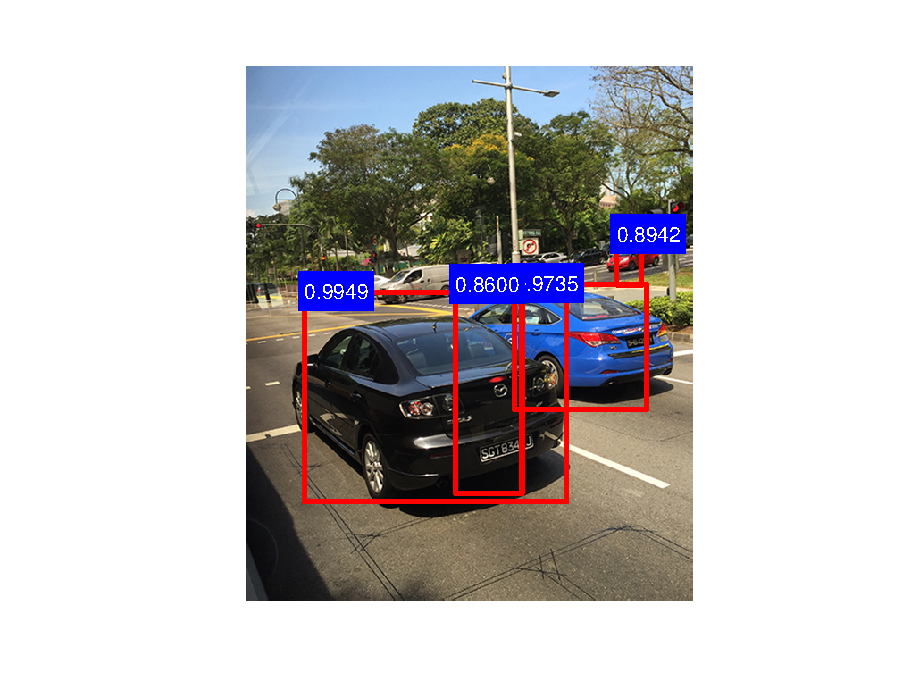
\includegraphics[width=4in, fbox]{Chapter1/boundingbox.eps}
\caption{Bounding-box example of cars.}
\label{fig:boundingboxexample} 
\end{figure}


\section{Motivation}

\lipsum[3]

\lipsum[4]


\section{Objectives and Specifications}



\section{Major contribution of the Dissertation}



\section{Organisation of the Dissertation}


\end{spacing}
%=== END OF CHAPTER ONE ===
\newpage


